\documentclass[11pt]{article}
\usepackage[margin=0.88in]{geometry}
\usepackage[T1]{fontenc}
\usepackage{lmodern}
\usepackage{amsmath,amssymb,amsthm,mathtools,booktabs,array,longtable}
\usepackage{graphicx,tikz,pgfplots}
\usetikzlibrary{arrows.meta,positioning,calc,fit}
\pgfplotsset{compat=1.18}
\usepackage{xcolor,microtype,enumitem}
\usepackage{hyperref}
\hypersetup{colorlinks=true,linkcolor=blue!45!black,citecolor=blue!45!black,urlcolor=blue!45!black,pdftitle={Agentic Progressive Optimization for Hardware-Software Co-Design of AI Infrastructure}}
\setlength{\parskip}{0.35em}
\setlength{\parindent}{0pt}
\setlength{\emergencystretch}{2em}
\renewcommand{\topfraction}{0.85}
\renewcommand{\textfraction}{0.10}
\renewcommand{\floatpagefraction}{0.80}
\setlist[itemize]{topsep=3pt,itemsep=2pt,leftmargin=1.5em}
\setlist[enumerate]{topsep=3pt,itemsep=2pt,leftmargin=1.8em}
\newtheorem{proposition}{Proposition}
\newcommand{\cD}{\mathcal D}
\newcommand{\cW}{\mathcal W}
\newcommand{\cF}{\mathcal F}
\newcommand{\cR}{\mathcal R}
\newcommand{\ind}{\mathbf 1}
\definecolor{ink}{HTML}{26364B}
\definecolor{softblue}{HTML}{EDF3FA}
\definecolor{softpurple}{HTML}{F2EFF7}
\definecolor{softgreen}{HTML}{EDF5F0}
\definecolor{blueedge}{HTML}{527FB1}
\definecolor{purpleedge}{HTML}{776292}
\definecolor{greenedge}{HTML}{42846A}
\tikzset{block/.style={draw=blueedge,fill=softblue,rounded corners=2pt,line width=.65pt,align=center,font=\footnotesize,inner sep=5pt},agent/.style={block,draw=purpleedge,fill=softpurple},eval/.style={block,draw=greenedge,fill=softgreen},flow/.style={-{Stealth[length=2mm]},draw=ink,line width=.7pt},feedback/.style={flow,dashed,draw=greenedge},labeltext/.style={font=\scriptsize,align=center,fill=white,inner sep=2pt}}
\title{Agentic Progressive Optimization for Hardware--Software Co-Design of AI Infrastructure}
\author{Research manuscript}
\date{October 9, 2026}
\begin{document}
\maketitle
\begin{abstract}
AI infrastructure design couples algorithms, software mappings, instruction interfaces, and hardware resources. A fixed representation can exclude valuable implementations, while a sufficiently expressive mixed-integer program can be prohibitively difficult to solve. We propose \textbf{Agentic Progressive Co-Design}, a framework that treats the construction of the design space and the search within it as connected optimization tasks. Starting from workload semantics, agents introduce algorithmic and hardware mechanisms, expose tensor-level dependencies, and compile their interactions into mixed-integer formulations. They then restructure the formulations, select coupled neighborhoods, and retain alternatives whose value depends on unresolved hardware choices. A common design assignment drives software lowering and hardware configuration; implementation feedback identifies which representation, cost model, or search decision to revise. We develop the formulation through streaming attention and explicit software--hardware boundary choices. Ventus case studies show why these mechanisms matter: a larger computation tile becomes beneficial only with a matching register organization, a previously unfavorable attention mapping becomes useful on another architecture, and fusion preferences reverse across hardware configurations. In a controlled calibrated study, joint selection reduces prefill and decode objectives by 10.84\% and 22.01\% relative to the baseline; decode improves by a further 4.10\% over one-pass software-first optimization. Iterative alternating optimization reaches the same objective in that menu. The evidence establishes concrete cross-layer opportunities and motivates a design process that expands what can be expressed while concentrating the optimization effort needed to realize it.
\end{abstract}
\section{Introduction}
A hardware resource has value only through the programs that use it. Larger tiles can reduce repeated weight transfers, yet increase register demand enough to reduce occupancy. More local storage can enable reuse, yet consume area that could support additional execution units or outstanding memory requests. Fusing two operators can remove intermediate transfers, yet change the instruction mix and the resources that limit progress. These choices jointly determine the efficiency of AI infrastructure.

The interactions are visible even within a small design family. In a Ventus study, increasing a matrix-multiplication tile from $32\times64$ to $64\times64$ reduced repeated weight traffic, but the new kernel required 173 vector registers. It performed poorly on the preceding register configuration and became useful after the hardware allocation changed. An attention mapping rejected on the default machine subsequently improved execution on another configuration~\cite{ventus-tiling}. Such reversals expose a limitation of committing to software or hardware choices before their interactions are understood.

Layered design makes a large problem manageable. A computation graph describes operators, a compiler constructs programs, an instruction interface specifies executable operations, and a hardware implementation supplies resources. Each layer hides details that other layers need not routinely consider. However, a hidden detail can become a consequential design variable. A coarse attention graph specifies matrix multiplication and normalization without exposing whether the score matrix is materialized, which tiles remain live, or how partial normalization state is updated. Once these choices become explicit, the available algorithms and the hardware needed to run them can change together.

This leads to two connected difficulties. \emph{Representation} determines which designs can be considered. An optimizer cannot select an online reduction, a different communication pattern, or a specialized data path that its representation does not admit. \emph{Search} determines which of the admitted designs can be found within the available effort. Expressing all relevant tiling, storage, scheduling, instruction, and hardware choices at once can produce a mixed-integer program (MIP) with an impractical number of variables and weak relaxations. Improving only one side leaves the other as a bottleneck.

We propose \textbf{Agentic Progressive Co-Design}: agents construct and revise the mathematical design problem, while optimization solvers search its explicit choices. The overall domain includes algorithmic organization, executable programs, the software--hardware boundary, and hardware structure. The active formulation exposes a selected part of that domain. Agents can introduce a new algorithmic family, expand a resource abstraction, derive a stronger encoding, or reopen a group of coupled decisions. They retain the assumptions behind reductions so that an unfavorable result on one machine does not eliminate a useful implementation elsewhere.

Three foundations suggest how to organize this process. CoSA shows how regular computation and architectural constraints support MIP-based scheduling~\cite{cosa}. Axon demonstrates semantics-driven generation of tensor-program alternatives and instruction implementations~\cite{axon}. LLM4MIP demonstrates a complementary role for language models in analyzing difficult optimization instances and developing primal and dual strategies~\cite{llm4mip}. Our framework connects these directions around a changing software--hardware design domain: the program family, hardware capabilities, and optimization representation can all be revised.

The software--hardware boundary is an explicit part of that domain. A transfer pipeline may be orchestrated by software, exposed through programmable asynchronous instructions, or managed by a specialized controller. These alternatives change instruction overhead, queue requirements, control area, and the range of workloads supported. Choosing among them requires the same joint treatment as choosing tile dimensions and memory capacity. The objective is a matched implementation: an algorithm and program organization, an execution interface, and a hardware structure that together satisfy the workload and deployment constraints.

Our contributions are:
\begin{itemize}
\item \textbf{A formulation of progressive design-space construction.} We distinguish the full bounded implementation domain from the designs represented by an active MIP, characterize expansion and restriction, and state conditions for hardware-dependent dominance and valid branch exclusion.
\item \textbf{A method for constructing and searching coupled formulations.} We connect algorithmic transformations, tensor dependencies, resource supply and demand, and boundary choices to linear encodings and paired software/hardware lowering. An agent policy distinguishes missing designs, weak formulations, and inaccurate cost models.
\item \textbf{An empirical analysis of cross-layer design mechanisms.} Ventus case studies connect register capacity, tiling, fusion, cache behavior, and memory concurrency to design quality. Controlled comparisons separate gains from co-design from gains attributable to a particular search strategy, and a model-error case shows why implementation feedback must influence subsequent formulation choices.
\end{itemize}

The mathematical framework and attention example describe the proposed method. The experiments exercise executable software alternatives, parameterized hardware models, and MIP-guided selection. They provide evidence for the cross-layer mechanisms on which the method relies; evaluation of autonomous formulation construction and generated instruction interfaces is a separate next step. Throughout, functional acceptance is a prerequisite for design evaluation. The subject of this paper is how to construct and optimize the design space.

\section{Related Work}
\textbf{Mathematical optimization of program decisions.}
CoSA encodes spatial and temporal scheduling choices for DNN accelerators as a MIP, using algorithmic and architectural constraints~\cite{cosa}. It provides a concrete basis for turning loop structure and resource limits into solver decisions. Checkmate uses mixed-integer optimization for tensor rematerialization~\cite{checkmate}, while COSMA jointly optimizes operator scheduling, memory allocation, and tensor replacement for a specified scratchpad capacity~\cite{cosma}. These systems demonstrate that decisions often handled by compiler heuristics can be represented mathematically. Our focus is how the program families, hardware resources, and interfaces underlying such decisions can evolve together, and how the formulation should change when those alternatives become relevant.

\textbf{Generating and representing optimized tensor programs.}
MLIR supports multiple abstraction levels and domain-specific intermediate representations~\cite{mlir}. TensorIR makes tensor computation primitives explicit within a compiler representation~\cite{tensorir}. Ansor searches generated tensor-program schedules using measurement and a learned cost model~\cite{ansor}. Mirage represents programs at kernel, thread-block, and thread levels to search combinations of algebraic and scheduling transformations~\cite{mirage}. These approaches establish that the representation is a central part of optimization: it determines the transformations that can be combined and the dependencies that remain visible.

Axon is particularly relevant to software-space construction. It generates tensor-graph alternatives, synthesizes target instruction sequences from semantics, and explores tiling and fusion for tile-based accelerators~\cite{axon}. Its persistent representation retains alternatives through successive stages. These capabilities suggest a source of implementation families for a global co-design formulation. Our design additionally exposes hardware resources and the implementation location of selected mechanisms as decisions. The generated family therefore has both software requirements and hardware realizations, rather than being ranked only on one target machine.

\textbf{Joint architecture and mapping search.}
DiGamma searches hardware and software mappings with a domain-aware genetic algorithm~\cite{digamma}. DOSA uses differentiable performance models to explore mappings and hardware together~\cite{dosa}. These works are direct precedents for joint optimization; hardware--software co-design itself is an established problem. We investigate a different control layer: how agents introduce design mechanisms, revise mathematical representations, and select structured subproblems. A fair evaluation must compare against strong joint and alternating search, in addition to one-pass layer-wise optimization.

\textbf{Language models and optimization formulations.}
OptiMUS constructs and solves mathematical optimization models from problem descriptions~\cite{optimus}. FormuEvo searches for solver-efficient formulations using language-model proposals and solver feedback~\cite{formuevo}. LLM4MIP studies already formulated MIP instances and uses structural analysis to develop feasible solutions and stronger bounds~\cite{llm4mip}. These directions motivate a formulation agent that reasons about dependent choices and auxiliary variables instead of directly predicting a large assignment. Co-design adds two responsibilities: discovering implementation choices that the current model does not express, and comparing the model's ranking with execution evidence. LLM4MIP is cited here as a research website and released workflow, whose technical report is forthcoming at the time of writing.

\textbf{Hardware generation and evaluation.}
Timeloop evaluates accelerator architectures and mappings~\cite{timeloop}; Gemmini connects a parameterized accelerator generator with its software stack~\cite{gemmini}; FireSim supports FPGA-accelerated system simulation~\cite{firesim}. Such infrastructure provides the realization and evaluation paths required after optimization. It also supplies information that a compact MIP may omit, including compiler resource allocation and shared-resource timing. Our framework uses this feedback to revise representation and cost assumptions. Its functional acceptance interface can employ existing checking tools, without making proof construction or proof reuse part of the optimization contribution.

\section{Co-Design as Progressive Design-Space Construction}\label{sec:space}
\subsection{Workloads, implementations, and a shared machine}
Let $\cW$ be a finite set of deployment scenarios. A scenario specifies the required computation, tensor dimensions, data types, permitted numerical error, and persistent state. Prefill and a bounded sequence of decoding steps are separate scenarios, even when they use the same model weights. The workload fixes the required outputs; it leaves implementation choices open.

A design is
\begin{equation}
 d=\bigl(h,b,\{a_w,p_w,m_w,\sigma_w\}_{w\in\cW}\bigr),\label{eq:design}
\end{equation}
where $h$ is the hardware structure, $b$ its software-visible boundary, $a_w$ an algorithmic organization, $p_w$ a program, $m_w$ its mapping, and $\sigma_w$ its execution organization. Hardware and interface choices are shared across scenarios. Programs and schedules can differ. This separates specialization to one shape from building a machine that must support several shapes or execution modes.

The implementation domain $\cD$ is bounded by a declared vocabulary: permitted arithmetic primitives, transformation families, storage structures, interface mechanisms, parameter ranges, and program-size limits. A design belongs to $\cD_W\subseteq\cD$ when its programs meet the workload contract and its hardware and execution satisfy the deployment constraints. A representative objective is
\begin{equation}
 \min_{d\in\cD_W} J(d),\qquad
 J(d)=\max_{w\in\cW}\frac{L_w(d)}{L_w^{\mathrm{ref}}},\quad
 A(h,b)\le A_{\max},\label{eq:objective}
\end{equation}
with fixed positive reference latencies. Energy, throughput, or weighted latency can replace this objective. Retaining programmability can be expressed through required scenario coverage or supported capabilities. For a single fixed workload, specialization is a legitimate outcome unless flexibility has an explicit value or constraint.

The joint domain can be viewed as one large mixed-integer design problem once the structural vocabulary and numerical approximations are fixed. This view does not require materializing that formulation in full. The computational task is to expose and solve useful portions while retaining the links needed to combine their decisions.

\subsection{Representations determine the reachable designs}
An active formulation is
\begin{equation}
 F_k=(R_k,X_k,C_k,\widehat J_k,D_k),\qquad
 \cF_k=\{x\in X_k:C_k(x)\},\label{eq:formulation}
\end{equation}
where $R_k$ is the representation, $X_k$ the variable domain, $C_k$ the constraints, $\widehat J_k$ the modeled objective, and $D_k$ a decoder into implementations. Its realizable set is $\cR_k=D_k(\cF_k)$. A decoder retains the identities of the selected software and hardware objects; a feasible assignment must be lowerable under the corresponding implementation contracts.

A coarse representation can describe a broad mathematical computation while providing a narrow set of executable lowerings. For example, an attention node denotes many possible implementations, but a backend that always materializes its score matrix cannot generate a streaming implementation. Refinement exposes state and dependencies that make another lowering expressible. It need not change the required computation.

There are four distinct modifications of an active model:
\begin{itemize}
\item \emph{Representation expansion} introduces additional realizable designs, such as an online reduction or a programmable transfer mechanism.
\item \emph{Equivalent reformulation} changes the encoding while preserving the decoded feasible designs and their objective values.
\item \emph{Restriction} removes a subset of designs through a justified dominance rule or a temporary search decision.
\item \emph{Cost or mechanism revision} changes the predicted behavior, constraints, or resource interactions associated with designs.
\end{itemize}
These operations need not produce nested feasible sets. Adding a new implementation family expands the design domain; modeling a previously omitted port conflict can remove assignments; changing coefficients can alter the ranking without changing feasibility. The system records these effects separately.

\begin{proposition}[Expansion under a fixed evaluator]\label{prop:expansion}
Suppose $\cR_k\subseteq\cR_{k+1}\subseteq\cD_W$, both sets are nonempty, and the same objective $J$ is used. Then
$\min_{d\in\cR_{k+1}}J(d)\le\min_{d\in\cR_k}J(d)$.
\end{proposition}
\begin{proof}
Every design admitted before expansion remains a candidate afterward, including any minimizer of the original finite design set.
\end{proof}
The proposition describes representational opportunity, not the quality achieved by a time-limited search. A richer representation can have a better optimum and still be harder to search. This distinction motivates retaining accepted incumbents and controlling where detail is introduced.

A useful decomposition separates the losses caused by representation, search, and prediction. Let $J^*=\min_{d\in\cD_W}J(d)$ and $J_k^*=\min_{d\in\cR_k}J(d)$. The representation loss is $J_k^*-J^*$. It is unaffected by additional solver effort within an unchanged $\cR_k$.

\begin{proposition}[Three sources of design loss]\label{prop:loss}
Let $\cR_k\subseteq\cD_W$ be finite and nonempty. Suppose $|\widehat J_k(d)-J(d)|\le\epsilon_k$ for every $d\in\cR_k$, and the selected design $\widehat d_k$ satisfies
$\widehat J_k(\widehat d_k)\le\min_{d\in\cR_k}\widehat J_k(d)+\delta_k$.
Then
\begin{equation}
 J(\widehat d_k)-J^*
 \le \underbrace{J_k^*-J^*}_{\text{representation loss}}
 +\underbrace{\delta_k}_{\text{optimization error}}
 +\underbrace{2\epsilon_k}_{\text{prediction error}}.\label{eq:loss}
\end{equation}
\end{proposition}
\begin{proof}
For a true minimizer $d_k^*$ over $\cR_k$,
$J(\widehat d_k)\le\widehat J_k(\widehat d_k)+\epsilon_k
\le\widehat J_k(d_k^*)+\delta_k+\epsilon_k
\le J_k^*+\delta_k+2\epsilon_k$.
Subtracting $J^*$ gives the result.
\end{proof}

This standard perturbation argument clarifies the agent's different responsibilities. Introducing a missing algorithm can reduce representation loss; stronger formulations or better search can reduce optimization error; implementation feedback can improve prediction. The quantities need not be known globally to guide experiments. A formal use of the bound, however, requires a uniform error guarantee; residuals on a sampled set alone do not provide one. The Ventus model-error case illustrates why a small $\delta_k$ can coexist with a poor realized design.

\subsection{Conditional dominance and alternative retention}
Dominance is a property of a design in context. Let $p$ and $q$ be two program fragments with the same functional interface, and let $\Gamma$ be a set of hardware configurations and surrounding programs. Removing $p$ is safe only when every feasible completion using $p$ in $\Gamma$ has a feasible completion using $q$ with no larger objective. Lower latency for one isolated kernel on one machine is insufficient: replacement can change storage lifetimes, interference, or other consumers' readiness.

\begin{proposition}[Contextual replacement]\label{prop:dominance}
For every feasible design $d$ using $p$ in a context in $\Gamma$, suppose a replacement $\rho(d)$ using $q$ preserves the required interface, remains feasible, and satisfies $J(\rho(d))\le J(d)$. Removing the $p$ designs in $\Gamma$ preserves the minimum objective over that domain.
\end{proposition}
\begin{proof}
The restricted set is a subset of the original set, so its optimum cannot improve. The replacement maps each removed design to a retained design with no worse objective, so its optimum cannot worsen.
\end{proof}

The useful engineering consequence is the scope of the rule. A dominance fact learned for one register budget or cache organization is stored with those conditions. A hardware change outside that context reopens the alternative. When the replacement conditions are only empirically suggested, exclusion is a heuristic search restriction and the branch remains available for reconsideration.

\subsection{The software--hardware boundary as a variable}
A boundary choice specifies which functions are fixed in hardware and which remain programmable. For a mechanism $j$, let $b_{j\mu}$ select one implementation mode $\mu$: a software sequence, a programmable instruction mechanism, or a specialized controller. The modes share an external functional interface but have different hardware requirements and lowering rules. We impose
\begin{equation}
 b_{j\mu}\in\{0,1\},\qquad \sum_{\mu\in M_j}b_{j\mu}=1.\label{eq:boundary}
\end{equation}
The choice may alter control area, instruction count, legal schedules, and supported tensor layouts. A capability is counted once in hardware and can serve many program regions. Each use pays its execution and contention costs.

This representation makes an otherwise fixed interface negotiable within an explicit library. It also distinguishes architectural sizing from boundary design: increasing queue depth changes capacity; introducing a completion-event interface changes what software can express. Both can be optimized, but they are different design decisions and require different implementation artifacts.

\section{Constructing Coupled MIP Formulations}\label{sec:construction}
\subsection{From computation graphs to implementation families}
Figure~\ref{fig:framework} shows the proposed organization. A representation hierarchy connects workload semantics to algorithmic organizations, tensor programs, instruction interfaces, and hardware structure. The hierarchy supports local detail: a region whose performance is well characterized can remain a compact implementation family while a contentious region exposes its transfers, buffers, and individual resource demands.

\begin{figure}[!t]
\centering
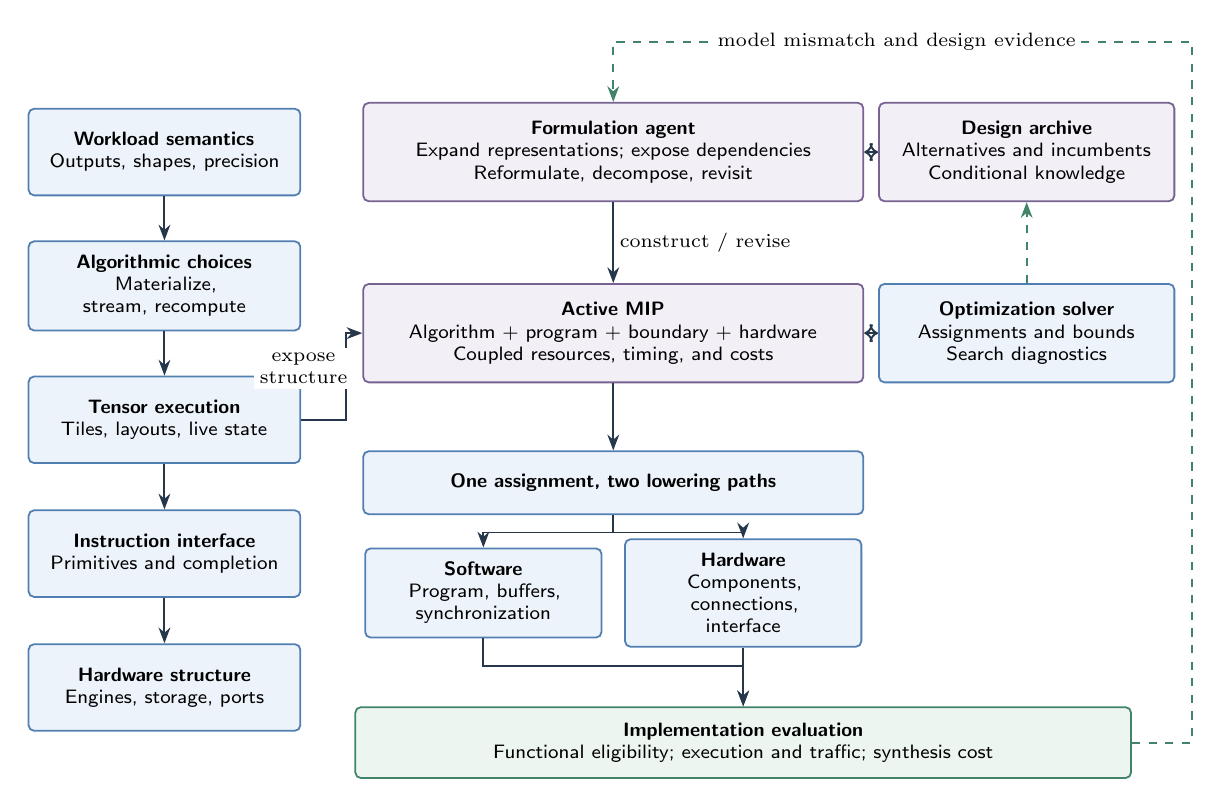
\begin{tikzpicture}[x=1cm,y=1cm,every node/.append style={font=\sffamily\scriptsize}]
\node[block,font=\sffamily\scriptsize,text width=3.1cm,minimum height=1.1cm] (w) at (1.65,8.2) {\textbf{Workload semantics}\\Outputs, shapes, precision};
\node[block,font=\sffamily\scriptsize,text width=3.1cm,minimum height=1.1cm] (a) at (1.65,6.5) {\textbf{Algorithmic choices}\\Materialize, stream, recompute};
\node[block,font=\sffamily\scriptsize,text width=3.1cm,minimum height=1.1cm] (t) at (1.65,4.8) {\textbf{Tensor execution}\\Tiles, layouts, live state};
\node[block,font=\sffamily\scriptsize,text width=3.1cm,minimum height=1.1cm] (b) at (1.65,3.1) {\textbf{Instruction interface}\\Primitives and completion};
\node[block,font=\sffamily\scriptsize,text width=3.1cm,minimum height=1.1cm] (h) at (1.65,1.4) {\textbf{Hardware structure}\\Engines, storage, ports};
\foreach \s/\d in {w/a,a/t,t/b,b/h}{\draw[flow] (\s.south)--(\d.north);}
\node[agent,font=\sffamily\scriptsize,text width=6cm,minimum height=1.25cm] (agent) at (7.35,8.2) {\textbf{Formulation agent}\\Expand representations; expose dependencies\\Reformulate, decompose, revisit};
\node[agent,font=\sffamily\scriptsize,text width=3.4cm,minimum height=1.25cm] (archive) at (12.6,8.2) {\textbf{Design archive}\\Alternatives and incumbents\\Conditional knowledge};
\draw[flow,<->] (agent.east)--(archive.west);
\node[agent,font=\sffamily\scriptsize,text width=6cm,minimum height=1.25cm] (mip) at (7.35,5.9) {\textbf{Active MIP}\\Algorithm + program + boundary + hardware\\Coupled resources, timing, and costs};
\draw[flow] (agent.south)--node[labeltext,right]{construct / revise}(mip.north);
\draw[flow] (t.east)--(3.95,4.8)--(3.95,5.9)--(mip.west);
\node[labeltext,anchor=east] at (4.05,5.45) {expose\\structure};
\node[block,font=\sffamily\scriptsize,text width=3.4cm,minimum height=1.25cm] (solver) at (12.6,5.9) {\textbf{Optimization solver}\\Assignments and bounds\\Search diagnostics};
\draw[flow,<->] (mip.east)--(solver.west);
\draw[feedback] (solver.north)--(archive.south);
\node[block,font=\sffamily\scriptsize,text width=6cm,minimum height=.8cm] (decode) at (7.35,4) {\textbf{One assignment, two lowering paths}};
\draw[flow] (mip.south)--(decode.north);
\node[block,font=\sffamily\scriptsize,text width=2.65cm,minimum height=1.05cm] (sw) at (5.7,2.6) {\textbf{Software}\\Program, buffers,\\synchronization};
\node[block,font=\sffamily\scriptsize,text width=2.65cm,minimum height=1.05cm] (hw) at (9,2.6) {\textbf{Hardware}\\Components, connections,\\interface};
\draw[flow] (decode.south)--++(0,-.22)-|(sw.north);
\draw[flow] (decode.south)--++(0,-.22)-|(hw.north);
\node[eval,font=\sffamily\scriptsize,text width=9.5cm,minimum height=.9cm] (eval) at (9,.7) {\textbf{Implementation evaluation}\\Functional eligibility; execution and traffic; synthesis cost};
\draw[flow] (sw.south)--++(0,-.35)-|(eval.north);
\draw[flow] (hw.south)--(eval.north);
\draw[feedback] (eval.east)--(14.7,.7)--(14.7,9.6)--(7.35,9.6)--(agent.north);
\node[labeltext] at (10.95,9.6) {model mismatch and design evidence};
\end{tikzpicture}
\caption{The proposed co-design loop. Representation levels on the left expose selected implementation choices; they do not prescribe an irreversible lowering order. Agents expand design capability and concentrate search. The same assignment determines software and hardware, and implementation evidence returns to the formulation policy.}\label{fig:framework}
\end{figure}


A \emph{family} is a parameterized implementation recipe. It specifies the computation it covers, external inputs and outputs, internal index and reduction structure, required capabilities, resource demand, and software and hardware lowering hooks. Parameters can include tile shape, buffering depth, layout, execution order, and instruction mechanism. Families can come from an established algorithmic library, compiler transformations, semantics-driven synthesis, or agent proposals admitted by the functional acceptance interface.

The agent's task includes identifying when the current families omit a relevant optimization paradigm. A model with only independent matrix multiplications cannot discover cross-operator streaming by adjusting their durations. A family must first expose the state and ordering that realize streaming. Hardware generation follows the same principle: choosing a specialized epilogue requires a component description and a corresponding program interface. A name attached to a binary decision variable does not supply its implementation.

Representation refinement therefore has two outputs. It adds executable structures, and it adds the relationships needed to price and constrain their combinations. Moving from graph-level edges to tensor slices reveals which values can be consumed early, which must remain live, and which can be recomputed. Moving from aggregate bandwidth to ports and queues reveals whether the proposed overlap is achievable. These relationships are the inputs to MIP construction.

\subsection{Worked example: exposing streaming attention}\label{sec:attention}
Consider one attention head with query length $N_q$, key length $N_k$, and feature dimension $d$:
\begin{equation}
 O=\operatorname{softmax}\!\left(QK^\top/\sqrt d+M\right)V,\label{eq:attention}
\end{equation}
where $M$ is a mask and every output row has at least one unmasked key. A graph-level implementation may materialize both scores and probabilities. A streaming family partitions queries into row blocks $I$ and keys/values into blocks $J$. Its state contains a running row maximum $m$, normalization denominator $\ell$, and unnormalized output accumulator $Z$. For a score block $S=Q_IK_J^\top/\sqrt d+M_{IJ}$, the update is
\begin{align}
 m' &= \max(m,\operatorname{rowmax}(S)), &
 \alpha &= \exp(m-m'), \nonumber\\
 P &= \exp(S-m'), &
 \ell' &= \alpha\odot\ell+\operatorname{rowsum}(P),\label{eq:online}\\
 Z' &= \operatorname{diag}(\alpha)Z+PV_J.\nonumber
\end{align}
After the final key block, $O_I=\operatorname{diag}(\ell)^{-1}Z$. For each row, its first block containing an unmasked key initializes the state; blocks with no valid contribution leave that row's state unchanged. This is the established online-attention organization underlying IO-aware attention~\cite{flashattention}; it is an example of a family to introduce, not a new attention identity.

The representation now exposes dependencies hidden inside the softmax node. Updating $Z$ requires both the previous accumulator and the new rescaling factor. A score tile can be released after its contribution to normalization and output is complete. The output accumulator remains live across key blocks. Loading the next $K,V$ block can overlap computation only when storage, transfer slots, and completion semantics support it. Work partitioning can further trade occupancy against shared-memory traffic, as illustrated by FlashAttention-2~\cite{flashattention2}.

\begin{figure}[tbp]
\centering
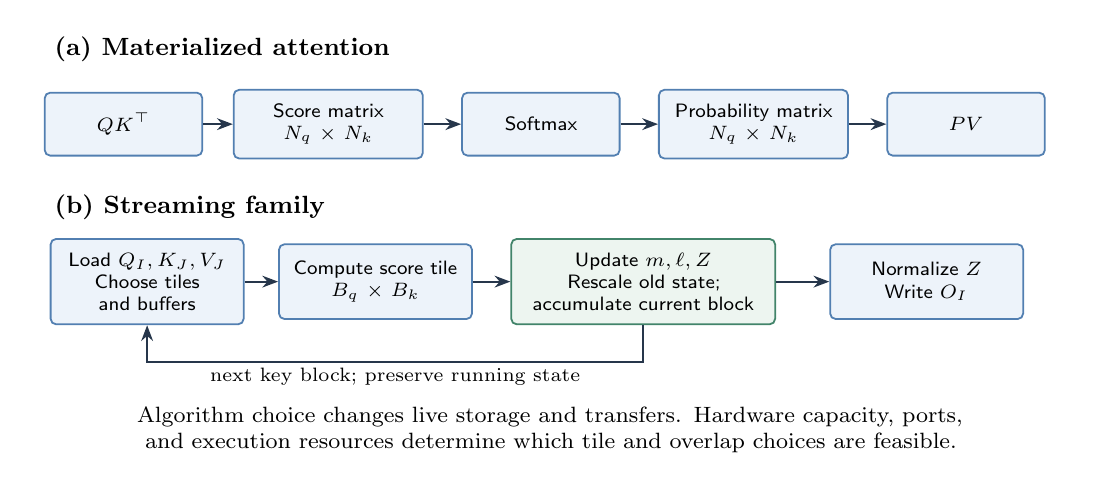
\begin{tikzpicture}[x=1cm,y=1cm,block/.append style={font=\sffamily\scriptsize},eval/.append style={font=\sffamily\scriptsize}]
\node[font=\small\bfseries,anchor=west] at (0,3.75) {(a) Materialized attention};
\node[block,text width=1.65cm,minimum height=.8cm] (qk) at (1,2.8) {$QK^\top$};
\node[block,text width=2.05cm,minimum height=.8cm] (s) at (3.6,2.8) {Score matrix\\$N_q\times N_k$};
\node[block,text width=1.65cm,minimum height=.8cm] (soft) at (6.3,2.8) {Softmax};
\node[block,text width=2.05cm,minimum height=.8cm] (p) at (9,2.8) {Probability matrix\\$N_q\times N_k$};
\node[block,text width=1.65cm,minimum height=.8cm] (pv) at (11.7,2.8) {$PV$};
\foreach \s/\d in {qk/s,s/soft,soft/p,p/pv}{\draw[flow] (\s.east)--(\d.west);}
\node[font=\small\bfseries,anchor=west] at (0,1.75) {(b) Streaming family};
\node[block,text width=2.1cm,minimum height=.95cm] (load) at (1.3,.8) {Load $Q_I,K_J,V_J$\\Choose tiles and buffers};
\node[block,text width=2.1cm,minimum height=.95cm] (score) at (4.2,.8) {Compute score tile\\$B_q\times B_k$};
\node[eval,text width=3cm,minimum height=.95cm] (state) at (7.6,.8) {Update $m,\ell,Z$\\Rescale old state;\\accumulate current block};
\node[block,text width=2.1cm,minimum height=.95cm] (out) at (11.2,.8) {Normalize $Z$\\Write $O_I$};
\foreach \s/\d in {load/score,score/state,state/out}{\draw[flow] (\s.east)--(\d.west);}
\draw[flow] (state.south)--(7.6,-.22)--node[labeltext,below]{next key block; preserve running state}(1.3,-.22)--(load.south);
\node[font=\footnotesize,align=center,text width=13cm] at (6.4,-1.08) {Algorithm choice changes live storage and transfers. Hardware capacity, ports, and execution resources determine which tile and overlap choices are feasible.};
\end{tikzpicture}
\caption{Exposing an algorithmic alternative requires new state and dependencies. The streaming recurrence avoids full intermediate matrices, while tile sizes, input reuse, buffering, and hardware support remain joint decisions.}\label{fig:attention}
\end{figure}


For a tile with $B_q$ query rows and $B_k$ key rows, a conservative local working-set estimate is
\begin{equation}
 B_{\mathrm{local}}=
 s_QB_qd+\nu(s_K+s_V)B_kd+s_SB_qB_k+s_ZB_qd
 +2s_rB_q,\label{eq:attention-storage}
\end{equation}
where $s_*$ are byte widths, $\nu$ is the number of buffered $K,V$ blocks, and $s_r$ is the running-statistic width. This expression assumes one score/probability buffer reused in place and excludes backend-specific scratch, alignment, and register spills, which the implementation family adds. Alternative reuse schedules produce different signatures. Byte counts should be distributed across the actual memory levels rather than charged to a single capacity if the lowering separates registers and shared memory.

For a fixed-query-block loop order, the $K,V$ stream is traversed once per query block unless another level captures reuse. Hence reducing intermediate materialization does not imply that all input traffic is read once. Query grouping, cache behavior, and buffer capacity remain optimization decisions. At fixed tile and hardware modes, the storage and traffic expressions become coefficients; their joint selection remains in the MIP.

This example defines a progression from a coarse operator graph to an algorithmic family and then a resource-constrained execution structure. It also gives a concrete expressiveness test: the representation should generate both materialized and streaming variants and allow the optimizer to select between them under different resource budgets.

\subsection{A finite linear encoding of coupled choices}\label{sec:encoding}
We give a compact encoding for a bounded design domain. Let $u$ index required semantic units, $r$ candidate regions, $c\in C_r$ their implementations, $i$ hardware slots, and $p\in P_i$ configurations for each slot. A slot may denote an engine, a memory component, or a parameterized subsystem. Local nonlinear expressions are evaluated for finite parameter combinations or represented with explicit linearization. They are not inserted into the MILP as unresolved products of design variables.

\textbf{Coverage and selection.}
Let $q_{rc}\in\{0,1\}$ select an implementation. For candidate regions covering a common semantic decomposition,
\begin{equation}
 \sum_{r,c:\,u\in\operatorname{cover}(r,c)}q_{rc}=1,
 \qquad \sum_{c\in C_r}q_{rc}\le1.\label{eq:cover}
\end{equation}
These constraints select a nonoverlapping cover. Algebraically different organizations need a preceding family selection: each selected family activates its own internal decomposition. A materialized softmax graph and an online-state recurrence must not be forced to share artificial one-to-one internal nodes. Their common interface is the attention result, while their internal constraints are conditional on the selected family.

\textbf{Hardware supply and implementation compatibility.}
Let $y_{ip}\in\{0,1\}$ select at most one configuration per slot, with $\sum_{p\in P_i}y_{ip}\le1$; an explicit absent mode can instead complete a one-hot selection. Resource supply and area can be written
\begin{equation}
 \operatorname{Cap}_h(y)=\sum_{i,p}K_{iph}y_{ip},\qquad
 A(y,b)=A_0+\sum_{i,p}A_{ip}y_{ip}+\sum_{j,\mu}A^{B}_{j\mu}b_{j\mu}.
 \label{eq:supply}
\end{equation}
The component partition assigns each physical cost once; boundary-specific controller area is excluded from $A_{ip}$ if it appears in $A^B$. Shared components are selected globally. For a required capability $g$, a selected implementation satisfies
\begin{equation}
 q_{rc}\le\sum_{i,p:\,g\in\operatorname{cap}(i,p)}y_{ip}.\label{eq:capability}
\end{equation}
This establishes presence. Binding and cumulative demand constraints determine whether that capability has enough instances and service capacity. If placement or topology matters, bindings identify the instance that executes each operation, and transfers must connect its producer and consumer memories.

\textbf{Timing and shared resources.}
For a time-indexed formulation, $x_{rct}=1$ starts implementation $(r,c)$ at tick $t$, with $\sum_t x_{rct}=q_{rc}$. Its duration $d_{rc}$ and resource profile $U_{rch}(\delta)$ are fixed for that implementation mode. Then
\begin{equation}
 \sum_{r,c,t}U_{rch}(\tau-t)x_{rct}
 \le \operatorname{Cap}_h(y) \quad\text{for every }h,\tau.\label{eq:resource}
\end{equation}
The profile can include overlapping compute, transfer, and epilogue stages. A hardware choice that changes latency must select a corresponding performance mode; it cannot silently change a coefficient after optimization. When contention changes operation order, the formulation introduces event ordering or a scheduling subproblem instead of assuming a fixed isolated duration captures that interaction.

Let $s_r=\sum_{c,t}t x_{rct}$ and $f_r=\sum_{c,t}(t+d_{rc})x_{rct}$. If selected producer $r$ and consumer $r'$ exchange a value, their activation variable $g_{rr'}$ enables
\begin{equation}
 s_{r'}\ge f_r+\delta_{rr'}-H(1-g_{rr'}),\label{eq:precedence}
\end{equation}
where $\delta_{rr'}$ is an explicitly charged transfer or visibility delay and $H$ is a valid bound for deactivation. The activation is linked to both selected endpoints and the chosen data path. Fusion can remove an external transfer while retaining its internal dependency. Streaming permits tile-level consumers to start before the whole region completes, using tile events instead of this coarse edge.

\textbf{Storage, ports, and overlap.}
A value-residency variable $\ell_{v\tau}$ is linked to the production and last consumption of value $v$. For fixed-size value objects,
\begin{equation}
 \sum_v B_v\ell_{v\tau}+\sum_{r,c,t}S_{rc}(\tau-t)x_{rct}
 \le\operatorname{Cap}_{\mathrm{mem}}(y),\label{eq:storage}
\end{equation}
where $S_{rc}$ accounts for internal scratch not already counted as external values. The compiler determines which operands occupy registers, shared memory, or external storage, and analogous inequalities apply separately to each level. Port demand and outstanding transfers consume separate resources. Two buffers create room for overlap; they do not establish that the ports or queues can sustain it.

\textbf{Objectives and multiple scenarios.}
For each scenario, $L_w$ bounds the completion of its required outputs, including final visibility. With the objective in Equation~\eqref{eq:objective}, a linear epigraph uses $T\ge L_w/L_w^{\mathrm{ref}}$ and minimizes $T$. Each scenario has its own program variables and shares $y,b$. Area and configuration limits constrain the common machine. Dynamic energy requires per-action or activity-aware coefficients; variable power multiplied by variable runtime requires another linearization or external evaluation. Clock frequency must likewise be fixed or tied to an evaluated hardware mode when comparing time rather than cycles.

\subsection{Encoding movable boundaries}\label{sec:boundary-example}
Figure~\ref{fig:boundary} illustrates a transfer mechanism. Software-controlled blocking loads, a programmable asynchronous interface, and a specialized streaming controller can implement the same data-flow requirement. They expose different choices to the program and consume different hardware resources.

\begin{figure}[tbp]
\centering
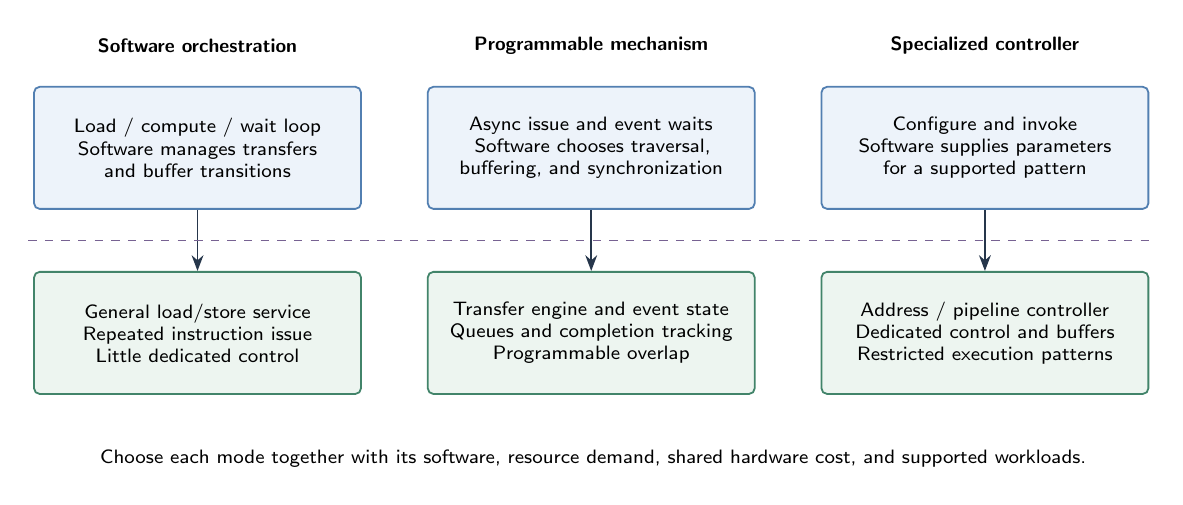
\begin{tikzpicture}[x=1cm,y=1cm]
\foreach \x/\title in {2.15/Software orchestration,7.15/Programmable mechanism,12.15/Specialized controller}{\node[font=\sffamily\scriptsize\bfseries,align=center] at (\x,4.65) {\title};}
\node[block,font=\sffamily\scriptsize,text width=3.8cm,minimum height=1.55cm] (s1) at (2.15,3.35) {Load / compute / wait loop\\Software manages transfers\\and buffer transitions};
\node[block,font=\sffamily\scriptsize,text width=3.8cm,minimum height=1.55cm] (s2) at (7.15,3.35) {Async issue and event waits\\Software chooses traversal,\\buffering, and synchronization};
\node[block,font=\sffamily\scriptsize,text width=3.8cm,minimum height=1.55cm] (s3) at (12.15,3.35) {Configure and invoke\\Software supplies parameters\\for a supported pattern};
\node[eval,font=\sffamily\scriptsize,text width=3.8cm,minimum height=1.55cm] (h1) at (2.15,1) {General load/store service\\Repeated instruction issue\\Little dedicated control};
\node[eval,font=\sffamily\scriptsize,text width=3.8cm,minimum height=1.55cm] (h2) at (7.15,1) {Transfer engine and event state\\Queues and completion tracking\\Programmable overlap};
\node[eval,font=\sffamily\scriptsize,text width=3.8cm,minimum height=1.55cm] (h3) at (12.15,1) {Address / pipeline controller\\Dedicated control and buffers\\Restricted execution patterns};
\foreach \n in {1,2,3}{\draw[flow] (s\n.south)--(h\n.north);}
\draw[dashed,draw=purpleedge] (0,2.17)--(14.3,2.17);
\node[font=\sffamily\scriptsize,align=center,text width=13.8cm] at (7.15,-.6) {Choose each mode together with its software, resource demand, shared hardware cost, and supported workloads.};
\end{tikzpicture}
\caption{Three possible locations of transfer-control functionality. Each mode has a different software-visible contract and hardware realization. The optimization prices the remaining programmability through the workloads and capabilities that the design must support.}\label{fig:boundary}
\end{figure}


An asynchronous implementation family requires the corresponding boundary mode, a compatible transfer engine, enough in-flight slots, and a buffer lifetime spanning completion. A specialized controller may reduce repeated instruction issue but accept only particular traversal patterns. The model links these choices with implications such as $q_{rc}\le\sum_{\mu\in M_{rc}}b_{j\mu}$ and resource constraints for every active transfer. Choosing a mode also selects its lowering recipe. For instance, a programmable mode emits completion events and waits; a controller mode emits configuration and invocation commands.

The same construction applies to reductions, layout conversion, or fused epilogues. Hardware specialization pays a shared area cost, whereas software retains freedom at a recurring instruction and scheduling cost. The optimization compares these costs across all required scenarios. Appendix~\ref{app:boundary} gives a complete finite encoding of this choice, including configuration-dependent execution costs.

\subsection{Decoding one assignment into paired implementations}
The decoder creates a software execution plan and a hardware configuration from the same selected objects. The execution plan specifies loop structure, addresses, buffer ownership, transfers, resource bindings, and synchronization. The hardware description specifies component instances, capacities, connections, and enabled interface mechanisms. A common identifier binds each emitted instruction capability to the implementing component.

For a parameterized existing architecture, the hardware output is a configuration of that generator. For a new boundary mechanism, the implementation library must also provide its controller or data path. The software backend cannot assume a mechanism that the hardware generator does not instantiate. Compilation then provides actual register and scratch requirements, which may differ from estimates used in the first model. Execution and synthesis return timing and implementation costs for the same paired design. These results close the loop by updating the family coefficients or exposing a missing constraint.

\section{Agent-Guided Reformulation and Search}\label{sec:search}
\subsection{The agent operates on design decisions and model structure}
The proposed agent receives the current representation, a typed mapping from variables to design objects, solver diagnostics, and implementation evidence. It produces a model action with an explicit scope. The action identifies which designs are added or restricted, which assumptions change, how an existing incumbent is reconstructed, and which evaluation can resolve the next uncertainty. This preserves the meaning of decisions when an encoding introduces many auxiliary variables.

The action space contains three groups. \emph{Construction actions} add algorithmic families, expose tensor dependencies, or introduce hardware capabilities. \emph{Reformulation actions} strengthen bounds, remove redundant variables, break valid symmetries, or choose a decomposition. \emph{Search actions} release a coupled neighborhood, revisit a branch, select a warm start, or allocate an implementation evaluation. Cost-model revisions accompany these actions when the execution evidence changes the ranking assumptions.

This division matters operationally. A weak lower bound calls for a stronger mathematical representation. A fast solver repeatedly selecting slow implementations calls for a better performance model or a missing design family. A capacity failure after compilation calls for a resource constraint or another lowering. These observations should not all trigger a larger random search.

\subsection{Structural reduction and coupled neighborhoods}
Many variables in a detailed MIP are consequences of a smaller set of structural decisions. A selected tile, buffer organization, interface mode, and hardware allocation determine much of the remaining transfer and schedule structure. The agent can search this semantic core while a completion problem assigns times, memory slots, or detailed bindings.

A useful neighborhood releases decisions connected by a mechanism. For a register-limited matrix multiplication, these can include tile shape, registers per multiprocessor, resident workgroups, tensor shape, and the area allocated to other storage. Releasing only tile size may find no improvement because the enabling hardware change remains fixed. Releasing only register capacity may appear wasteful because the software does not exploit it. The neighborhood should preserve their coupling while fixing unrelated choices.

The formulation can exploit additional structure. Identical engine instances admit symmetry-breaking orderings if the workload and connectivity treat them interchangeably. Factorized loop mappings can avoid enumerating full schedules. Valid working-set inequalities can eliminate impossible combinations before introducing time-indexed variables. Derived demand variables can replace repeated expressions, and bounded binary--continuous products can use standard linearization. Each transformation is justified with respect to its declared domain; an instance-specific observation is not promoted to a universal rule.

\subsection{Decomposition, completion, and bounds}
A natural master problem chooses hardware, interface modes, and algorithmic families. Scenario subproblems choose detailed programs and schedules on that shared machine. This decomposition is useful when the master captures the strong global interactions and each scenario can otherwise be completed independently. Simultaneous multi-scenario execution requires a shared contention subproblem rather than independent completion.

A failed completion returns information about the combination that failed. If an exact subproblem proves a particular structural assignment infeasible, a no-good constraint can exclude that assignment. A stronger conflict cut can exclude a larger set only when its derivation supports that scope. A compiler error or a timed-out scheduling attempt does not establish infeasibility of every possible implementation with those high-level choices.

Primal and dual progress have different roles. A completed design gives a feasible objective for its evaluator. A solver lower bound applies to its formulation. For a branch $B$, a valid bound $\underline J_B\le\inf_{d\in B}J(d)$ permits pruning when $\underline J_B\ge U$, where $U$ is an accepted incumbent under the same objective and evaluator. An analytic model can support that statement if it is a certified relaxation of the target evaluation. A fitted prediction without a one-sided guarantee supports prioritization, not this bound-based exclusion.

Equivalent reformulations can retain bound meaning through a known mapping. Expanding the candidate family can invalidate a lower bound for the previously restricted problem; changing latency coefficients changes the objective being bounded. The archive therefore indexes bounds by model identity and scope. This prevents an inexpensive local optimum from being treated as a conclusion about the full design domain.

\subsection{Retaining and revisiting alternatives}
The candidate archive stores accepted implementations, unresolved family branches, and contextual knowledge. Structural signatures describe algorithmic organization, reuse direction, storage placement, boundary mode, and hardware allocation. Retention can then preserve distinct possibilities rather than many parameter variations of the same design.

An accepted design remains an incumbent when the representation expands, provided its workload and implementation conditions remain valid. A rejected design has a reason: illegal semantics, a resource violation, a provably dominated context, or an unfavorable evaluation. Only the last category is a performance judgment, and its scope includes the hardware and workload on which it was made. The packed-attention reversal in Section~\ref{sec:tiling-results} illustrates why this distinction matters.

The archive also supports conditional knowledge reuse. A statement such as ``this tile reuses a weight panel until register pressure reduces occupancy'' contains a mechanism and applicability conditions. It can guide another scenario's initial formulation while leaving the threshold to be recomputed. A statement such as ``larger tiles are always better'' discards the conditions needed for transfer.

\subsection{Feedback-driven action selection}
The agent diagnoses three types of disagreement. \emph{Feasibility disagreement} occurs when a modeled design cannot be lowered or violates a realized resource limit. \emph{Ranking disagreement} occurs when implementation evaluation changes the ordering of candidates. \emph{Search disagreement} occurs when a promising represented family remains difficult to explore despite an adequate evaluator. The responses are respectively to repair the interface or constraint, revise the relevant cost mechanism, or restructure the optimization.

Evaluation effort is directed toward decisions that can change the selected design. For example, two nearly tied memory organizations may justify detailed simulation of their contention, while a capacity-infeasible candidate can be removed analytically. When error bars are empirically estimated, they guide this allocation without becoming mathematical bounds. Expensive evaluations should include both promising designs and discriminating alternatives that test the agent's explanation of the bottleneck.

The procedure below specifies the proposed control loop. Its policy can begin with explicit rules and language-model proposals; a learned action policy is an optional implementation of the same interface.

\begin{quote}
\small
\textbf{Progressive co-design procedure}\par
\textbf{Input:} workload set, component and transformation library, budgets, initial representation, and exploration budget.\par
1. Build an initial formulation and preserve a feasible reference design.\par
2. Diagnose missing families, solver difficulty, and implementation-model mismatch from the current record.\par
3. Propose a scoped construction, reformulation, or search action; retain its assumptions and reconstruction map.\par
4. Solve the active MIP or master/completion subproblems. Keep feasible assignments, bounds, and termination status.\par
5. Decode selected assignments into paired software and hardware. Check functional and resource eligibility, then evaluate execution and implementation cost.\par
6. Update coefficients, mechanism constraints, and contextual knowledge. Retain competitive structural alternatives and reopen affected branches.\par
7. Repeat while the exploration budget permits; return the best eligible evaluated design and its model-specific optimization information.
\end{quote}

An evaluation of the agent should count the entire loop: formulation construction, language-model inference, solver calls, failed compilations, simulation, and synthesis. Solver time alone can improve while total exploration becomes more expensive. Conversely, an expensive model revision can be worthwhile when it is reused across many workload shapes. These are distinct amortization questions.

\section{Experimental Evaluation}\label{sec:evaluation}
\subsection{Questions, workloads, and evaluation scope}
The case studies address three questions: (1) do software choices change value when hardware changes; (2) what does joint selection gain over fixed or sequential design; and (3) when does the optimization model fail to predict realized behavior? They use a Ventus-derived architecture model with compiled instruction streams, software variants, and parameterized compute, memory, and service resources~\cite{ventus-controlled,ventus-tiling,ventus-model}. The evaluation is organized by these questions rather than by the individual exploration runs.

P128 and P512 denote prefill with 128 and 512 tokens. D128 and D512 denote the mean cycle count over 16 decoding steps starting at the corresponding context length. For each scenario $w$, $r_w=L_w/L_w^{\mathrm{ref}}$ compares a candidate with the same study's fixed baseline. Prefill, decode, and combined objectives take the maximum ratio over their respective scenario sets, as in Equation~\eqref{eq:objective}. A lower ratio is better; a cycle reduction of $1-r$ differs from a speedup of $1/r$.

The controlled fusion study uses Qwen2.5-14B-Instruct with 48 layers, batch one, BF16 operands and storage, and FP32 accumulation. Its 35.52\,mm$^2$ modeled budget uses a fixed ideal resource-replication factor of 32. Whole-network values are calibrated estimates assembled from compiled representative programs, with packing, layout conversion, intermediate movement, bias, and the final language-model head charged. The smaller-network tiling and model-fidelity studies use a 1.11\,mm$^2$ estimated area budget and complete instruction-timing simulations of their selected scenarios. These studies have different evaluators and baselines; their ratios are interpreted within each study.

The evidence evaluates cross-layer mechanisms and bounded MIP-guided selections. The instruction simulator models control, addresses, and resource timing; it does not compute complete inference tensors. Resource and workload-coverage checks accompany the timing results, and numerical checks have a separate local scope. Area is modeled and the results are cycle-based, without a common-frequency physical implementation study. The experiments do not evaluate an autonomous agent producing the entire representation hierarchy. Source snapshots, normalization definitions, and plotted values are provided with the manuscript artifact.

\subsection{Fusion preferences reverse across hardware}\label{sec:fusion-results}
Consider the D128 gate/up projection representative program in the controlled study. On the baseline hardware H0, the fused implementation takes 2.750761 million cycles, compared with 2.918714 million for separate execution. On U3, the separate implementation takes 2.510624 million cycles, while the fused implementation takes 2.762451 million. Fusion is therefore approximately 5.75\% faster on H0; separation is approximately 9.12\% faster on U3. Figure~\ref{fig:controlled}a shows the reversal~\cite{ventus-controlled}.

U3 reallocates the area budget. Relative to H0, it reduces scalar-register slots from 2048 to 128 and local data storage from 128 to 16\,KiB per multiprocessor, while increasing L1 miss-status entries from four to eight and load/store entries from eight to sixteen. Both configurations retain 64 multiprocessors, 1024 vector-register slots, and tensor shape $(4,8,4)$. The measured pair therefore changes more than a scalar throughput parameter: software organization interacts with service concurrency and storage allocation.

This is a direct test of contextual dominance. A rule that permanently removes the separate implementation after evaluating H0 excludes the faster U3 program. The correct knowledge is conditional on the hardware and execution context. A formulation can retain both implementations and link their resource demands and timing coefficients to the selected machine, or a search procedure can reopen the software choice after changing hardware.

\begin{figure}[tbp]
\centering
\begin{tikzpicture}
\begin{axis}[width=6.7cm,height=5.6cm,ybar,bar width=13pt,ymin=0,ymax=3.5,ytick={0,1,2,3},ylabel={Million cycles},symbolic x coords={H0,U3},xtick=data,enlarge x limits=.5,title={(a) Fusion preference reversal},title style={font=\small},tick label style={font=\footnotesize},label style={font=\footnotesize},legend style={font=\scriptsize,at={(.5,-.31)},anchor=north,legend columns=2,draw=none},ymajorgrids,grid style={gray!15}]
\addplot[fill=blueedge!70,draw=blueedge] table[x=hardware,y=fused,col sep=comma] {evidence/fusion.csv};
\addplot[fill=greenedge!65,draw=greenedge] table[x=hardware,y=separate,col sep=comma] {evidence/fusion.csv};
\legend{Fused,Separate}
\end{axis}
\begin{axis}[at={(8.4cm,0)},anchor=south west,width=7.1cm,height=5.6cm,xbar,bar width=5pt,xmin=0,xmax=1.06,xtick={0,.25,.5,.75,1},xlabel={Worst normalized cycles},symbolic y coords={Alternating,Joint,SW then HW,HW only,SW only,Baseline},ytick=data,enlarge y limits=.12,title={(b) Controlled design strategies},title style={font=\small},tick label style={font=\scriptsize},label style={font=\footnotesize},legend style={font=\scriptsize,at={(.5,-.31)},anchor=north,legend columns=2,draw=none},xmajorgrids,grid style={gray!15}]
\addplot[fill=blueedge!70,draw=blueedge] table[x=prefill,y=method,col sep=comma] {evidence/controlled.csv};
\addplot[fill=greenedge!65,draw=greenedge] table[x=decode,y=method,col sep=comma] {evidence/controlled.csv};
\legend{Prefill,Decode}
\end{axis}
\end{tikzpicture}
\caption{Controlled Ventus study~\cite{ventus-controlled}. (a) D128 gate/up representative-program timing changes its preferred software organization across hardware. (b) Whole-network calibrated objectives use the same seven-configuration menu. Joint and iterative alternating selection tie. Lower is better in both panels; the panels use different units.}\label{fig:controlled}
\end{figure}


\subsection{Joint selection and the strength of the baseline}\label{sec:joint-results}
The same study compares baseline, software-only, hardware-only, one-pass software-first, joint, and iterative alternating optimization. The final common menu contains seven hardware configurations; software options include projection fusion, tiling, input packing, attention organization, and row-block dispatch. Each method accesses the same completed menu subject to its own fixed-choice restrictions. Alternating optimization repeatedly computes the best software response to the current hardware and the best hardware response to that software.

For prefill, joint selection reaches $r=0.891559$, a 10.84\% reduction from baseline. For decode, it reaches $r=0.779915$, a 22.01\% reduction. The one-pass software-first objectives are 0.895792 and 0.813232, respectively. Joint selection therefore adds 0.473\% prefill and 4.097\% decode improvement over that sequential procedure. Figure~\ref{fig:controlled}b shows all six strategies. The combined objective selects the same design as prefill~\cite{ventus-controlled}.

The hardware choices are also different across objectives. Prefill selects R072 at an estimated 34.4716\,mm$^2$, while decode selects U3 at 33.3117\,mm$^2$. R072 adds a second writeback port to the U3 organization. On the software side, 32-row dispatch groups improve some prefill projections while retaining the compiled kernel, packed input, and output layout. Paired checks preserve instruction, requested-byte, and matrix-operation counts. Some hardware configurations show little benefit or regress, so the optimizer retains the original dispatch where appropriate.

Iterative alternating optimization reaches the same objectives as joint selection in this menu. The experiment thus establishes the benefit of revisiting coupled decisions, and the loss from a single software-first pass, without attributing an exclusive advantage to the MIP algorithm. This is an informative outcome: when best-response updates suffice, a more elaborate search policy must justify its cost on a larger or more strongly coupled domain.

The selected software and hardware are held fixed for a second-backend evaluation. Prefill and decode reductions remain 10.191\% and 19.941\% relative to that backend's corresponding baselines. Both backends share parts of the instruction-decoding path, so this is a sensitivity check on the selected design. Separate cache-assumption variations produce prefill reductions between 10.66\% and 11.46\%. These ranges describe modeled scenarios rather than statistical confidence intervals.

\subsection{Tiling, registers, and the value of reopening a branch}\label{sec:tiling-results}
A complete-instruction-simulation study provides a complementary example of representation expansion. Its earlier prefill design uses three multiprocessors and tensor shape $(2,16,2)$, with a software mapping based on smaller matrix tiles. A $64\times64$ kernel is then introduced to reduce weight reloads relative to the $32\times64$ tile. The reported traffic analysis identifies repeated loading across query-row blocks, and the larger tile reduces that traffic by roughly one third~\cite{ventus-tiling}.

The new kernel requires 173 vector registers. On the preceding VGPR-512 hardware, the reported comparison worsens from 0.362 to 0.438 in normalized cycles. An alternative hardware organization uses two multiprocessors, tensor shape $(4,8,4)$, VGPR 1024, and a different cache allocation. The larger tile becomes useful in this context. Figure~\ref{fig:trajectory} traces the accepted prefill designs using their complete-simulation objectives.

A second reversal appears within the expanded family. Packed QK, previously unfavorable on the default machine, improves P512 from 0.377 to 0.334 on the new hardware. A subsequent L2 variation produces a design with estimated area 1.0812\,mm$^2$ and ratios 0.3417, 0.3308, 0.2953, and 0.2719 for P128, P512, D128, and D512. The combined objective is 0.3417, corresponding to approximately $2.93\times$ the baseline performance under this timing model. A separate decode-oriented design attains a decode objective near 0.279~\cite{ventus-tiling}.

\begin{figure}[tbp]
\centering
\begin{tikzpicture}
\begin{axis}[width=.89\linewidth,height=5.6cm,ymin=0,ymax=.45,ytick={0,.1,.2,.3,.4},ylabel={Prefill worst normalized cycles},symbolic x coords={Earlier,N3,N4},xtick=data,xticklabels={Earlier accepted design,New tile + hardware,L2 variant},enlarge x limits=.2,ybar,bar width=35pt,nodes near coords,point meta=y,nodes near coords style={font=\footnotesize},every node near coord/.append style={/pgf/number format/fixed,/pgf/number format/precision=4},tick label style={font=\footnotesize},label style={font=\footnotesize},ymajorgrids,grid style={gray!15}]
\addplot[fill=blueedge!65,draw=blueedge] table[x=design,y=prefill,col sep=comma] {evidence/trajectory.csv};
\end{axis}
\end{tikzpicture}
\caption{Accepted-design trajectory from complete instruction simulations. Introducing the larger-tile kernel and a matching register/tensor/cache configuration expands the available combination; an L2 variation then changes the selected hardware. The values are rounded as reported. This trajectory illustrates design evolution, rather than a controlled ablation of individual changes.}\label{fig:trajectory}
\end{figure}


The progression illustrates two operations in the proposed method. Introducing a larger-tile kernel expands the represented program family. Reopening register, tensor, and cache choices creates a coupled neighborhood in which that kernel becomes valuable. It would be misleading to describe this simply as choosing a larger tile or simply as adding registers. The useful object is the new software--hardware combination.

These results are an observed exploration trajectory. They do not isolate the effect of an automated retention policy, since the retained and discarded branches were not compared under a matched policy experiment. They do identify a concrete failure mode that such a policy must handle: a local rejection can become obsolete after a hardware change.

\subsection{A closed MIP gap can coexist with a poor design model}\label{sec:model-results}
The model-fidelity study uses Qwen2.5-0.5B-Instruct, 24 layers, two compiled software families, and a structured search over 27 hardware fields. Nine MIP solves report optimal solutions for their approximate models. Their predicted worst-scenario ratio is approximately 0.3333. Complete instruction simulation instead yields objectives between 0.7913 and 0.8987, a prediction shortfall of roughly 58--63\% relative to the simulated values~\cite{ventus-model}.

The optimization outcome follows the modeling error. Software-only selection retains the baseline software, and hardware-only designs match or outperform the joint selections. For prefill, the joint candidate has objective 0.8987, compared with 0.7913 for hardware-only selection. For the combined objective they tie at 0.8272. An earlier subgraph-selected configuration also outperforms these new candidates on the complete scenarios. The result locates the problem in the connection between model and execution, rather than in an unresolved branch-and-bound gap.

Transfer further exposes the scope of the learned design. Fixing the selected Qwen hardware and applying the corresponding software implementations to GPT-2 small and Pythia-160M produces cycle ratios of 3.07--5.60 relative to their own baselines. In the analyzed cases, the FFN down projection accounts for approximately 62--64\% of the additional cycles, and memory-read volume rises substantially while matched operation instruction counts remain unchanged~\cite{ventus-model}. The observation identifies where to refine the reuse and memory model; it does not isolate one hardware parameter as the cause.

For the proposed control loop, this pattern calls for mechanism and cost revision. Spending more time solving the same approximate MIP cannot correct its ranking. A useful next formulation would expose the mapping-dependent traffic and concurrency responsible for the discrepancy, preserve stronger evaluated designs, and restrict the applicability of any knowledge transferred from the original workload.

\subsection{What the studies establish}
Together, the cases establish three properties of the design problem. Software transformations have hardware-dependent value; a one-pass design process can leave useful combinations unexplored; and model fidelity determines whether mathematical optimization improves the realized design. They also show that sophisticated joint search does not automatically improve on a strong alternating method.

The results support the mechanism-level motivation for progressive co-design. Measuring the full agent policy requires a separate comparison in which candidate access, evaluator, and total exploration budget are controlled. Its outcomes should include design quality, number of costly evaluations, solver effort, and representation changes. The method's benefit would then be attributable to how it constructs and navigates the space, rather than to a larger unreported candidate library.

\section{Design Implications and Next Steps}
\subsection{From established paradigms to new combinations}
The first test of a design representation is whether it can express competitive existing implementations. Attention provides a useful progression: materialized scores, tiled fusion, online normalization, different work partitions, and hardware-supported data movement. The representation should expose the mechanisms that distinguish these families, allowing them to combine with hardware choices. Encoding the name of an existing kernel as one opaque option offers a useful baseline, but provides little opportunity to recombine its internal decisions.

A richer representation creates the possibility of improving on established designs; it does not establish that improvement by itself. A frontier comparison needs a current strong implementation for the same workload, precision, and target constraints. Software comparisons hold hardware fixed. System comparisons allow hardware changes under a common resource and implementation-cost model. Reporting both separates algorithmic gains from additional hardware capability. The Ventus studies establish useful combinations within their declared domains; a claim of performance beyond state-of-the-art implementations requires that additional comparison.

\subsection{How much of the boundary should move?}
A software--hardware boundary should be reopened when its fixed assumptions prevent a useful design or impose repeated overhead. Reopening every interface simultaneously makes both implementation and optimization harder. The proposed approach introduces explicit alternatives for a selected mechanism, retains their programmable degrees of freedom, and evaluates the consequences over the required workload set.

The current cases vary hardware resources and software organization within an existing interface. The boundary formulation in Section~\ref{sec:boundary-example} extends that domain. An implementation study of boundary movement should generate the competing controllers or instruction mechanisms, compile matching programs, and include area and timing costs under a common technology and clock methodology. This would test whether specialization's recurring performance benefit justifies its fixed cost and reduced flexibility.

\subsection{Cost fidelity and optimization scale}
Fine-grained timing, bank conflicts, and dynamic arbitration can overwhelm a global MILP. A compact master model with conditional resource signatures and selective detailed completion is one way to manage this scale. It introduces a modeling choice: which interactions can be summarized without changing important rankings? The model-fidelity case shows why this question needs execution evidence.

The quality of the implementation library also limits the domain. Compiler register allocation, unsupported layouts, and backend synchronization rules can change feasibility after an initial model is built. These effects should produce explicit family restrictions or refined estimates. Physical cost introduces additional interactions, including memory macros, wiring, frequency, and control logic. A logical-area estimate and a cycle count do not determine an implemented chip's energy or latency.

\subsection{Evaluating the agent and reusable knowledge}
An agent can improve the design space, the formulation, or the allocation of search effort. These effects require different controls. With a fixed final space, compare equivalent formulations and structured search against strong solver and heuristic baselines. With an evolving space, give policies access to the same transformation and component libraries, then measure which designs they expose and how much evaluation effort they spend. A retention ablation should revisit the conditional reversals seen in the case studies.

Knowledge transfer is also conditional. A mapping rule learned on one architecture can identify a promising mechanism elsewhere, but its performance threshold depends on the new resource ratios. The negative transfer case argues for storing those conditions and validating them on reserved workloads. Human intervention and model-inference costs belong in the accounting. Reusable formulation knowledge is valuable when its construction cost is amortized over enough related design problems.

\section{Conclusion}
AI infrastructure design joins algorithmic choices, programs, interfaces, and hardware into one coupled optimization problem. Its difficulty lies both in representing valuable implementations and in searching the resulting combinations. Agentic Progressive Co-Design addresses these tasks together: introduce the mechanisms needed to express a useful design, encode their interactions in a MIP, exploit structure to make search tractable, and use paired implementation feedback to revise the next model.

The Ventus studies show that hardware changes can reverse software preferences, that revisiting coupled choices improves on one-pass optimization, and that a closed solver gap cannot repair an inaccurate performance model. These findings motivate a design process in which abstraction boundaries and optimization formulations remain revisable. The resulting research direction is a systematic route from workload semantics to a matched algorithm, executable program, software--hardware interface, and hardware organization.

\begin{thebibliography}{99}
\bibitem{cosa} Q. Huang, M. Kang, G. Dinh, T. Norell, A. Kalaiah, J. Demmel, J. Wawrzynek, and Y. S. Shao. \emph{CoSA: Scheduling by Constrained Optimization for Spatial Accelerators}. ISCA, 2021. \url{https://arxiv.org/abs/2105.01898}.
\bibitem{axon} A. Kothari, S. Zhu, D. Kroening, and C. Sung. \emph{Axon: A Synthesizing Superoptimizer for Tensor Programs}. arXiv:2606.26344, 2026. \url{https://arxiv.org/abs/2606.26344}.
\bibitem{llm4mip} Y. Huang, W. Gao, D. Ge, M. Udell, and Y. Ye. \emph{How Much Can LLMs Help Solve MIPs?} Research website and released workflows, October 2026. Accessed October 9, 2026. \url{https://llm4mip.github.io/}.
\bibitem{checkmate} P. Jain et al. \emph{Checkmate: Breaking the Memory Wall with Optimal Tensor Rematerialization}. MLSys, 2020. \url{https://arxiv.org/abs/1910.02653}.
\bibitem{cosma} Y. Li, A. Gupta, and S. Malik. \emph{Combined Scheduling, Memory Allocation and Tensor Replacement for Minimizing Off-Chip Data Accesses of DNN Accelerators}. arXiv:2311.18246, 2023. \url{https://arxiv.org/abs/2311.18246}.
\bibitem{mlir} C. Lattner et al. \emph{MLIR: A Compiler Infrastructure for the End of Moore's Law}. arXiv:2002.11054, 2020. \url{https://arxiv.org/abs/2002.11054}.
\bibitem{tensorir} S. Feng et al. \emph{TensorIR: An Abstraction for Automatic Tensorized Program Optimization}. ASPLOS, 2023. \url{https://arxiv.org/abs/2207.04296}.
\bibitem{ansor} L. Zheng et al. \emph{Ansor: Generating High-Performance Tensor Programs for Deep Learning}. OSDI, 2020. \url{https://www.usenix.org/conference/osdi20/presentation/zheng}.
\bibitem{mirage} M. Wu et al. \emph{Mirage: A Multi-Level Superoptimizer for Tensor Programs}. OSDI, 2025. \url{https://www.usenix.org/conference/osdi25/presentation/wu-mengdi}.
\bibitem{digamma} S.-C. Kao et al. \emph{DiGamma: Domain-aware Genetic Algorithm for HW-Mapping Co-optimization for DNN Accelerators}. DATE, 2022. \url{https://arxiv.org/abs/2201.11220}.
\bibitem{dosa} C. Hong, Q. Huang, G. Dinh, M. Subedar, and Y. S. Shao. \emph{DOSA: Differentiable Model-Based One-Loop Search for DNN Accelerators}. MICRO, 2023. Author version: \url{https://arxiv.org/abs/2509.10702}.
\bibitem{optimus} A. AhmadiTeshnizi et al. \emph{OptiMUS-0.3: Using Large Language Models to Model and Solve Optimization Problems at Scale}. arXiv:2407.19633, version 4, 2026. \url{https://arxiv.org/abs/2407.19633}.
\bibitem{formuevo} H. Yuan, J. Peng, J. Bi, N. Zhang, S. Song, and Z. Cao. \emph{FormuEvo: LLM-Guided Evolution for Discovering Solver-Efficient Mixed-Integer Programming Formulations}. arXiv:2608.23353, 2026. \url{https://arxiv.org/abs/2608.23353}.
\bibitem{timeloop} A. Parashar et al. \emph{Timeloop: A Systematic Approach to DNN Accelerator Evaluation}. ISPASS, 2019. \url{https://accelergy.mit.edu/timeloop.pdf}.
\bibitem{gemmini} H. Genc et al. \emph{Gemmini: Enabling Systematic Deep-Learning Architecture Evaluation via Full-Stack Integration}. DAC, 2021. \url{https://people.eecs.berkeley.edu/~ysshao/assets/papers/genc2021-dac.pdf}.
\bibitem{firesim} S. Karandikar et al. \emph{FireSim: FPGA-Accelerated Cycle-Exact Scale-Out System Simulation in the Public Cloud}. ISCA, 2018. \url{https://fires.im/}.
\bibitem{flashattention} T. Dao, D. Y. Fu, S. Ermon, A. Rudra, and C. R\'e. \emph{FlashAttention: Fast and Memory-Efficient Exact Attention with IO-Awareness}. NeurIPS, 2022. \url{https://arxiv.org/abs/2205.14135}.
\bibitem{flashattention2} T. Dao. \emph{FlashAttention-2: Faster Attention with Better Parallelism and Work Partitioning}. ICLR, 2024. \url{https://arxiv.org/abs/2307.08691}.
\bibitem{ventus-controlled} Ventus Co-Design Project. \emph{Qwen2.5-14B Controlled Hardware--Software Optimization Study}. Public experiment report, issue 4, October 9, 2026. \url{https://github.com/BinaryCheater/ventus-codesign/issues/4}.
\bibitem{ventus-tiling} Ventus Co-Design Project. \emph{Tiling, Register Allocation, and Attention-Mapping Co-Design Study}. Public experiment report, issue 3 and updates through comment 6077879211, October 9, 2026. \url{https://github.com/BinaryCheater/ventus-codesign/issues/3}.
\bibitem{ventus-model} Ventus Co-Design Project. \emph{Qwen Full-Network Optimization and GPT-2/Pythia Transfer Study}. Public experiment report, issue 6, October 9, 2026. \url{https://github.com/BinaryCheater/ventus-codesign/issues/6}.
\end{thebibliography}

\appendix
\section{Notation and Linearization}\label{app:encoding}
Table~\ref{tab:notation} summarizes the objects used in the formulation. All finite ranges, time horizons, and coefficient versions are part of a model instance.

\begin{table}[htbp]
\centering\small
\begin{tabular}{p{.20\linewidth}p{.72\linewidth}}
\toprule
Symbol & Meaning \\
\midrule
$\cW,\cD_W$ & Required deployment scenarios and feasible bounded implementation domain \\
$R_k,\cF_k,\cR_k$ & Active representation, feasible assignments, and decoded realizable designs \\
$a,p,m,\sigma$ & Algorithmic organization, program, mapping, and execution organization \\
$h,b$ & Shared hardware structure and software-visible boundary choices \\
$q_{rc},x_{rct}$ & Implementation selection and time-indexed start decisions \\
$y_{ip},b_{j\mu}$ & Hardware-slot configuration and boundary-mode selection \\
$U_{rch},S_{rc}$ & Local resource-demand and internal-scratch profiles \\
$\ell_{v\tau},B_v$ & Value residency and fixed byte footprint \\
$L_w,\widehat J,J$ & Scenario latency, modeled objective, and target evaluator objective \\
\bottomrule
\end{tabular}
\caption{Main notation. A symbol denoting a program $p$ is distinct from the configuration index $p\in P_i$ in hardware-slot sums.}\label{tab:notation}
\end{table}

\textbf{Logical conjunction.}
For binary selections $q,y$, an auxiliary $z=q\land y$ is encoded by
\begin{equation}
 z\le q,\quad z\le y,\quad z\ge q+y-1,\quad z\ge0.
\end{equation}
This is useful for configuration-dependent duration or energy coefficients. It enumerates local interactions without requiring an opaque candidate for every whole-system combination.

\textbf{Binary--continuous products.}
For $z=qv$ with $q\in\{0,1\}$ and known bounds $L\le v\le U$, the exact linearization is
\begin{equation}
 Lq\le z\le Uq,\qquad v-U(1-q)\le z\le v-L(1-q).
\end{equation}
Tight bounds matter for relaxation strength. A generic large constant can make a valid model unnecessarily difficult to solve.

\textbf{Residency.}
Residency variables cannot be free capacity switches. For a selected implementation, they are constrained to remain active from production or preallocation until every required consumer completes. One finite encoding enumerates allowed start/last-use pairs and derives the active interval; another uses production and release events with cumulative conservation. Aliasing and buffer reuse require nonoverlapping live ranges or explicit ordering. Internal scratch and exported values must not be counted twice.

\textbf{Configuration-dependent timing.}
A single duration coefficient is valid only for the hardware conditions under which it was defined. A finite $(\text{implementation},\text{hardware mode})$ table can use conjunction variables. A factorized model instead represents the relevant service capacities explicitly and derives event times. The former is compact when interactions are local; the latter is needed when relative order and interference change with the configuration.

\textbf{Conditional families.}
Suppose an attention region has family selectors $g_{\mathrm{mat}},g_{\mathrm{stream}}$ summing to one. Each internal operation $u$ belonging to family $a$ satisfies $\sum_{r,c:\,u\in\operatorname{cover}_a(r,c)}q_{rc}=g_a$. The selected family exports the same region-level inputs and output. Transfers and lifetimes are internal to that family except for shared external values. This avoids treating an online recurrence as a cover of intermediate tensors that it intentionally does not materialize.

\section{A Complete Finite Boundary-Choice Model}\label{app:boundary}
Consider a region that must transfer and consume $N$ tiles in each workload scenario. Let $\mathcal H$ be a finite set of machine configurations and $\mathcal M=\{\mathrm{sw},\mathrm{async},\mathrm{ctrl}\}$ the permitted transfer-control modes. Each hardware/mode pair has a generator and compiler interface. Let $\mathcal C_w$ contain software variants with fixed tile sizes, traversal order, and buffering depth for scenario $w$.

The coefficients are: shared area $A_h$, incremental mode area $A^B_{h\mu}$, compatibility $K_{wh\mu c}\in\{0,1\}$, and evaluated or modeled latency $t_{wh\mu c}$. The mode-area coefficient includes only components not already counted in $A_h$. Compatibility includes numerical eligibility, supported traversal, live storage, resource demand, and interface support. Thus a specialized controller may support fewer variants than the programmable mode.

Choose binary hardware $y_h$, mode $b_\mu$, and software $q_{wc}$ variables with
\begin{equation}
 \sum_h y_h=1,\qquad \sum_\mu b_\mu=1,\qquad
 \sum_{c\in\mathcal C_w}q_{wc}=1\quad\forall w.
\end{equation}
Let $v_{h\mu}=y_h\land b_\mu$ and $z_{wh\mu c}=v_{h\mu}\land q_{wc}$ using the conjunction encoding above. The complete selection model is
\begin{align}
 \min\quad &T,\nonumber\\
 \text{subject to}\quad
 &z_{wh\mu c}\le K_{wh\mu c} &&\forall w,h,\mu,c,\nonumber\\
 &\sum_h A_hy_h+\sum_{h,\mu}A^B_{h\mu}v_{h\mu}\le A_{\max},\label{eq:finite-boundary}\\
 &L_w=\sum_{h,\mu,c}t_{wh\mu c}z_{wh\mu c} &&\forall w,\nonumber\\
 &T\ge L_w/L_w^{\mathrm{ref}} &&\forall w.\nonumber
\end{align}
Hardware and boundary mode are shared, while programs differ across scenarios. The area of an asynchronous engine is paid once even when several scenario programs use it. Its per-scenario effect is represented in $t$ and $K$. Latency entries must include startup, queue occupancy, synchronization, and the attainable overlap for the selected variant.

This finite model is an exact optimizer of its supplied table. Its purpose is to make the boundary decision and accounting explicit. Scaling to a large family replaces parts of the table with factorized resource and event constraints, and generates additional variants as needed. Doing so changes the computational representation while retaining the shared implementation identities. A boundary experiment would populate these coefficients from generated software and hardware; the empirical studies in Section~\ref{sec:evaluation} retain their existing instruction interface.

\section{Empirical Definitions and Source Records}\label{app:evidence}
The accompanying artifact stores the public source reports and comments as retrieved on October 9, 2026, alongside machine-readable data used in the figures. These are frozen report snapshots, not a substitute for executable experiment packages. The source reports identify the underlying branches and available reproduction material. No new accelerator simulation is required to reproduce the manuscript figures.

\textbf{Controlled study.}
The objectives in Figure~\ref{fig:controlled}b are the maximum normalized cycles across two prefill or two decode scenarios. In the order baseline, software-only, hardware-only, software-first, joint, and alternating, the prefill values are
$1$, $0.995747$, $0.908609$, $0.895792$, $0.891559$, and $0.891559$.
The decode values are
$1$, $0.816048$, $0.949019$, $0.813232$, $0.779915$, and $0.779915$.
The relative gain over software-first is $(r_{\mathrm{seq}}-r_{\mathrm{joint}})/r_{\mathrm{seq}}$.
The source is the controlled study~\cite{ventus-controlled}, with the snapshot retaining its update timestamp.

The study's acquisition domain contains 735 hardware profiles; seven configurations form the final evaluated selection menu. The report records 584 newly completed native evaluations and approximately 149.7 minutes of campaign wall time. Cache reuse and historical receipts increase the final data index to 1568 entries; that count is not the number of new simulations. The final menu's zero MIP gap describes its selection model. Representative-program aggregation, sampled decode steps, and ideal resource replication define the whole-network estimate.

\textbf{Tiling trajectory.}
Figure~\ref{fig:trajectory} uses the earlier accepted prefill objective 0.367 from the issue body, N3's rounded objective 0.342 from comment 6077807611, and N4's 0.3417 from comment 6077879211~\cite{ventus-tiling}. These are successive accepted designs, not equal-budget policy trials. The N4 ratios are $0.3417$, $0.3308$, $0.2953$, and $0.2719$; its estimated area is 1.0812\,mm$^2$. The figure preserves the precision available in each source entry.

\textbf{Model fidelity and transfer.}
The model study~\cite{ventus-model} uses complete Qwen instruction-timing runs and fixed-hardware transfer tests. Its software-only option remains the baseline software. The final configurations reported for transfer are the best designs among each task's specified controls, not necessarily the design labeled joint. GPT-2 small and Pythia-160M use FP16 software paths, whereas Qwen uses BF16. Their cycle ratios are normalized to the corresponding workload's own baseline, and are not pooled with the 14B calibrated study.

\end{document}
